%!TEX root = ../main.tex
\section{NSA Überwachung vs. Vorratsdatenspeicherung}
  \subsection{NSA Überwachung vs. Vorratsdatenspeicherung}
    \begin{frame}<beamer>{NSA Affäre}
      \begin{itemize}
        \item  Whistelblower und ehmaliger Geheimdienstmitarbeiter Edward Snowden 
        \item  seit 2007: Überwachung der Telekommunikation insbesondere  das Internet global und verdachtsunabhängig überwacht wird.
        \item  Rechtfertigung seitens der Politiker und Geheimdiensten ist die Bekämpfung des internationalen Terrorismus
        \item  Daten wurden auf Vorrat gespeichert
        \item  Gebäude und Vertretungen der UN und der Europäischen Union wurden mit Wanzen auspioniert
        \item  große Diplomatische Spannungen wurden verursacht
        \item  Bürgerrechtsorganisationen demonstrieren weltweit gegen Maßenüberwachung
      \end{itemize}
    \end{frame}
    \begin{frame}<beamer>{NSA Affäre vs. Vorratsdatenspeicherung}
      \begin{itemize}
        \item CDU und SPD sprechen sich gegen die NSA-Überwachung aus, treten jedoch noch immer für VDS ein
        \item CDU und SPD weigern sich Edward Snowden in Deutschland zum Überwachungsskandal zu befragen 
        \item 1. Mai 2014 Merkel Besuch in den USA
         \begin{itemize}
          \item Verbandspräsident Kurt Lauk (CDU): rät Merkel NSA Affäre zu vergessen (Quelle: Spiegel)
          \item Hauptargument: „Ich war da immer realistisch: Jeder spioniert gegen jeden"
          \item Lauk sieht im NSA Skandal nur eine technologische Überlegenheit der USA
          \item Ziel sollte technologischer Gleichstand sein
            \end{itemize}
      \end{itemize}
    \end{frame}
    \begin{frame}<beamer>{Danke für Ihre Aufmerksamkeit}
      \begin{itemize}
       \item Danke für Ihre Aufmerksamkeit
       \\
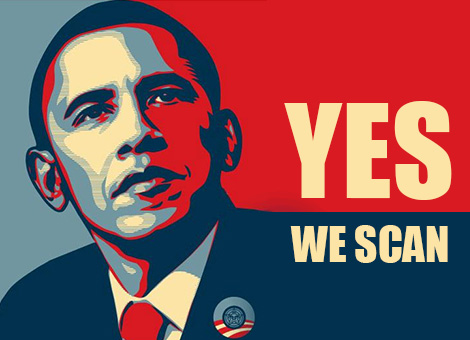
\includegraphics[height=0.75\textheight]{sections/img/yes-we-scan.jpg}
      \end{itemize}
    \end{frame}
 
